\chapter{Languages}

In order for a language to be at all useful it must \textit{mean something.}
Meaning is a difficult thing to grasp since in order to talk about
it at all it is necessary to use language which itself involves a
question of meaning. However, it is possible to set down some broad
ground-rules that can be used to establish a basic framework. 

First of all, a language has a syntax which comes in two flavours:
concrete and abstract. Concrete syntax is how you read or write a
language, it tends to be human-centric. The following is an example
of concrete syntax:

\begin{lstlisting}
x + 1
\end{lstlisting}
Abstract syntax deals with how a language is represented as data;
it tends to be computer-centric. Here is the equivalent example represented
as abstract syntax (think of the Java data structure that is created
rather than the characters making up the program):

\begin{lstlisting}
new BinExp(new Var("x"),PLUS,new Int(1))
\end{lstlisting}
In order to build systems we need a language with a syntax. Rather
than use any old language, this book is about constructing languages
that are a good fit for the required system. In doing so we need control
over the concrete syntax (to make it easy to work with for a human)
and control over the abstract syntax (to make it easy for a computer
to work with it).

The process by which concrete is turned into abstract syntax is called
\textit{parsing}. This book deals with models of languages and provides
a great deal of examples of grammars that specify how to turn concrete
into abstract syntax language representations.

Next, the syntax of a language does not define its meaning any more
than you can judge a book by its cover. In order to have meaning,
a language must have a \textit{semantic domain}. A semantic domain
is a model of the elements that the language denotes. A semantic domain
for natural language (such as English) contains all the real-world
concepts you can think of (such as Elephants and houses) in addition
to all the conceptual things you can think of; in fact, it contains
anything you can think of. 

Languages used for system development are much more controlled in
terms of syntax and semantics than natural languages. The semantic
domains of such languages are defined by data types for elements appropriate
to the systems domain. The particular data types depend on the system
domain, for example a language for expressing telecomms will have a
semantic domain containing networks, routers and devices. Languages
defined for general use have general purpose semantic domains containing
such things as records, integers, strings, events etc.

Finally, the meaning of a language is not defined by its syntax or
its semantics alone; the meaning is the \textit{mapping} that links
the syntax to the semantics. In terms of modelling languages the mapping
is often static, for example linking class definitions to sets of
objects that are the instances of the classes. This of UML-style class
models. What is the meaning of such a model? Since the class diagram
does not specify any behaviour, neither does the semantics. a suitable
semantics might be all the objects that can be constructed whose structure
matches that specified in the class model. For programming languages
the mapping is dynamic since it links programs to execution traces
and all the execution machinery that lives in the traces. 

To understand a language you must be fluent in its syntax, its semantic
domain and the mapping between them.

This book defines the super-language XMF and describes how you use
it to bridge the representation chasm. This book is \emph{not} about
how you analyse the systems themselves in order to model them; there
are plenty of books about that topic. This book aims to provide a
collection of techniques that allow you to raise the abstraction-bar
when addressing system development issues. 

When modelling systems it is desirable to focus on \emph{what} is
being expressed rather than \emph{how} the information is being represented.
This is the essence of a language driven approach: we can use high-level
abstractions to capture the information without worrying about unnecessary
implementation detail. The language that will be used to represent
the information in this book is designed to provide a wide range of
high-level constructs for modelling information. 

%
\begin{figure} \begin{center}
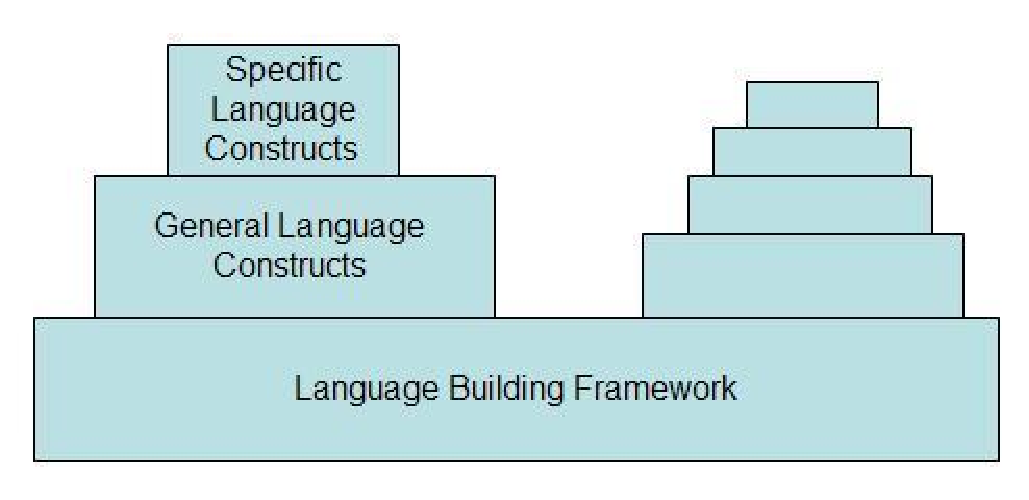
\includegraphics[width=12cm]{XMF/Languages/Images/Tower.pdf}
\caption{Towers of Languages\label{fig:Towers-of-Languages}}
\end{center} \end{figure}


Futhermore, the language has been specifically designed to be extensible:
if no language construct is provided to express the required information
then the user can extend the language with a new construct that does
the job. This is the \emph{ball-of-mud} model first pioneered by the
Lisp family of programming languages. Rather than being a pejorative
term, a language is like a ball of mud when new features can be added
to the language in a way that the new features become part of the
language and are indistinguishable from the existing features. No
special actions need to be taken to use the new extensions: they have
been seamlessly integrated into the language.

Rather than being a ball of mud, it is possible to view the different
languages as towers as shown in figure \ref{fig:Towers-of-Languages}.
The base level is a very general language that supports the construction
of other language (ideally it will support the definition of itself).
A language is grown from the basic framework by adding successive
layers of language constructs; each layer is built from all those
layers below it and the layers become progressively more tailored
to specific application domains. The ball of mud principle is maintained
when the addition of a layer does not preclude the use of constructs
from lower layers and when languages build in different towers can
be used in the same application.

This chapter defines the semantic domain for the language that is
used throughout the rest of the book. The next chapter describes the
syntax of the language XOCL. The chapter after than describes language
building features. On reading the rest of this chapter you should
expect to appreciate the key data values that can be expressed and
the kind of operations that are applied to the values. Each major
category of value has a section to itself.

The element types are divided into groups described in the following
sections. In each case the types that form a coherent aspect of the
semantic domain are grouped together. An overview of the aspect is
given along with a collection of operations that make up an interface
for the group. Note that the interface is very general; it is intended
that a given application will extend this interface by dynamically
adding more operations to the domain types as required. In addition,
the operations describes in each section are an overview. The gold
standard of operations for each type is the source code of XMF itself.


\section{Everything is an Element}

%
\begin{figure} \begin{center}
\hfill{}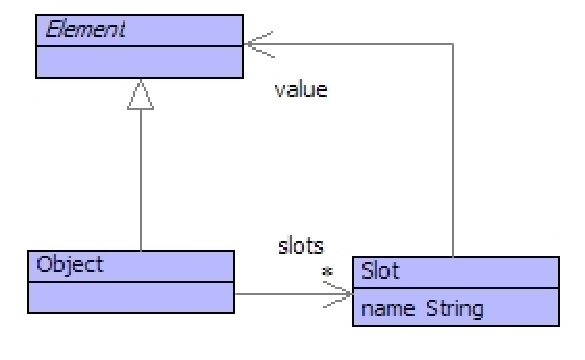
\includegraphics[width=8cm]{XMF/Languages/Images/Element.pdf}\hfill{}

\caption{Element and Object\label{fig:Element-and-Object}}

\end{center} \end{figure}


Figure \ref{fig:Element-and-Object} shows the root class of the value
domain: everything is an element - some things are objects. When designing
the value domain we had a choice: should everything be an object?
Objects have state represented as slots; a slot has a name and a value.
The slots of an object can be updated. Objects have an identity: when
you create an object it will be different to every other object that
you have ever created (even if the slots are the same).

But not all values have changeable state and an identity. For example:
the integer 3. Does it make sense to talk of the state of 3? Does
it make sense to change the state of 3? Given two occurrences of 3,
are they the same or not?

The distinction between Element and Object allows us to make the distinction
between values whose state cannot change and which have no identity.
Therefore, 3 is an element, but not an object. A set is an element
and not an object, as is a string and a boolean value.

Our language is object-oriented and computation proceeds by message
passing. When an element is sent a message, if its type defines an
operation with the same name as the message then the operation defines
the actions that are performed. If T defines an operation o expecting
arguments (x,y,z) then T::o(x,y,z) is the operation. In the rest of
this chapter each section defines some types; the key operations for
the types are described; where the type of arguments or the return
type of an operation is Element then the type is omitted.

The main operations defined by Element are:

\begin{lstlisting}
Element::copy()
  // Returns a copy of the receiver.
Element::equals(other):Boolean
  // Returns true when the arg is equal
  // to the receiver.
Element::init()
  // Initializes the receiver.
Element::isKindOf(type:Classifier):Boolean
  // Returns true when the receiver is an
  // instance of the supplied type.
Element::of():Classifier
  // Returns the type of the receiver.
Element::toString():String
  // Returns a string representation 
  // of the receiver.
\end{lstlisting}
The main operations defined by Object are:

\begin{lstlisting}
Object::get(name:String)
  // Return the value of the slot or throw
  // an error if the slot does not exist.
Object::hasSlot(name:String):Boolean
  // Returns true when the receiver has a
  // slot with the given name.
Object::set(name:String,value)
  // Updates the given slot or throws an
  // error if the slot does not exist.
\end{lstlisting}
\section{Indexing Things}

%
\begin{figure} \begin{center}
\hfill{}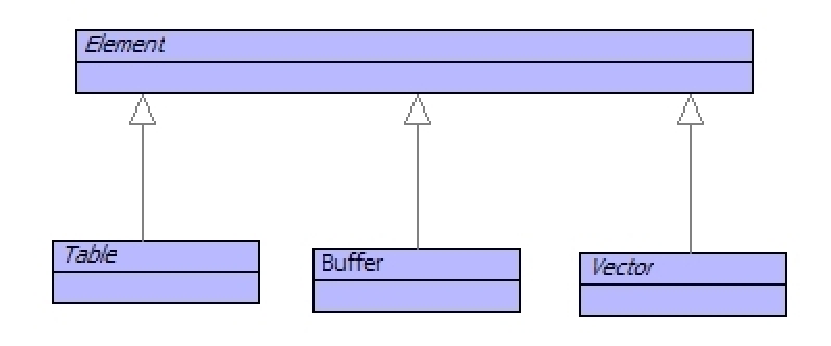
\includegraphics[width=12cm]{XMF/Languages/Images/Table.pdf}\hfill{}

\caption{Indexed Collections\label{fig:Indexed-Collections}}

\end{center} \end{figure}


When dealing with values it is desirable to build collections where
the elements in the collection are indexed by a key. The key is specified
when the element is placed into the collection and the key is used
to look the element up in the collection. The value associated with
a key in a collection may be changed. 

Figure \ref{fig:Indexed-Collections} shows three classes that are
used to represent basic indexed collections. Notice these classes
extend Element, not Object, therefore these indexed collections have
no slots. A table uses any element as a key, buffers and vectors use
integers as keys. The difference between a buffer and a vector is
that the former grows to accommodate elements as they are added whereas
the latter is a fixed size.

What would you use these for? A table is useful when building arbitrary
associations, for example associating names of personnel with their
employment records. Vectors are useful when you know the size of the
collection in advance, for example the locations on a chess board.
Buffers are useful when you need the collection to grow as required
and want to index elements by their position, for example building
an output string.

The main table operations are as follows:

\begin{lstlisting}
Table(n:Integer):Table
  // Returns a table. The argument indicates the
  // likely max keys.
Table::clear()
  // Empties the receiver.
Table::get(key)
  // Returns the value of the key or raises 
  // an error if the key is not present.
Table::hasKey(key):Boolean
  // Returns true when the key is in the table.
Table::keys():Set(Element)
  // Returns the keys in the table.
Table::put(key,value)
  // Updates the table.
Table::remove(key)
  // Removes the key from the table.
Table::values():Set(Element)
  // Returns the set of values in the table.
\end{lstlisting}
The main buffer operations are as follows:

\begin{lstlisting}
Buffer(n:Integer,isString:Boolean):Buffer
  // Returns a buffer. The first arg is the size to 
  // grow by each time the buffer is extended. The 
  // second indicates whether the buffer is a string 
  // buffer or a general buffer.
Buffer::add(element)
  // Adds the element to the end of the buffer.
Buffer::append(s:String)
  // Appends the chars to the end of a string buffer.
Buffer::asSeq():Seq(Element)
  // returns the buffer as a sequence.
Buffer::at(i:Integer)
  // Returns the element at index i or throws an error
  // if the buffer has no element at position i.
Buffer::size():Integer
  // Returns the number of elements currently in 
  // the buffer.
\end{lstlisting}
The main vector operations are:

\begin{lstlisting}
Vector(n:Integer):Vector
  // Returns a new vector of the specified size.
Vector::asSeq():Seq(Element)
  // Returns the vector as a sequence.
Vector::put(element,index:Integer)
  // Updates the vector at the specified index or
  // throws an error if the index is out of range.
Vector::ref(i:Integer)
  // Returns the element at the specified index.
Vector::size():Integer
  // Returns the size of the vector.
\end{lstlisting}
\section{Naming Things and Looking Them Up}

%
\begin{figure} \begin{center}
\hfill{}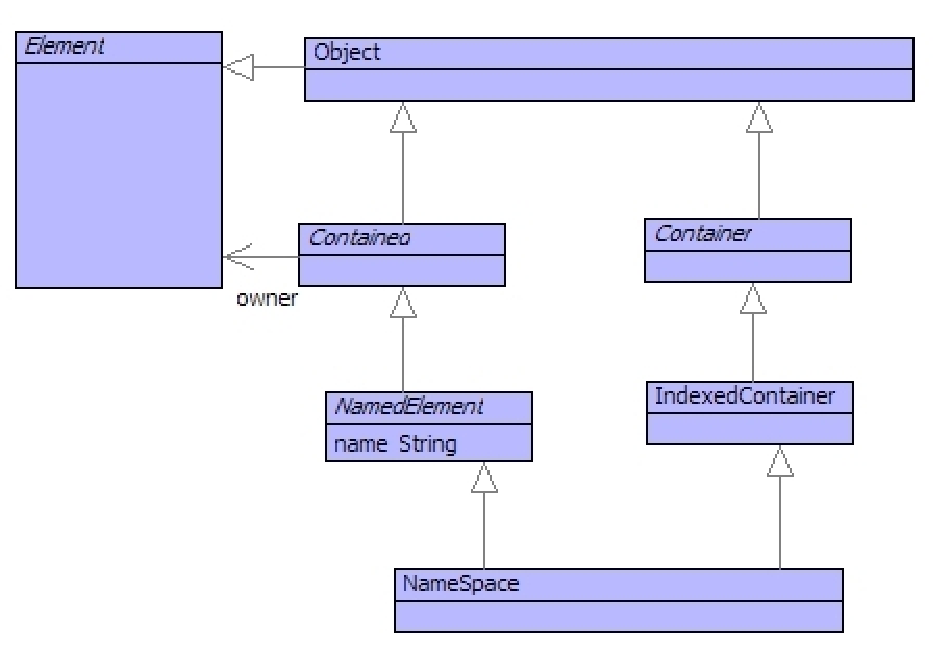
\includegraphics[width=12cm]{XMF/Languages/Images/NameSpace.pdf}\hfill{}

\caption{Named Elements live in Name Spaces\label{fig:Named-Elements-live}}

\end{center} \end{figure}


Elements are often identified by their name and the value domain provides
special support for named elements and their containers. Figure \ref{fig:Named-Elements-live}
shows the classes that define these elements. A contained element
has a link to its owner and a named element is a contained element
with a name. A container is a class that wraps up internal storage
implemented by tables, vectors and the like. An indexed container
is a wrapper for a table (allowing users to extend the class). A name
space is a named element that contains other named elements.

Notice that the structure of a name space allows name spaces to contain
other name spaces. This means that references to named elements may
cross a number of nested name spaces, leading to the idea of a \emph{path}
to an element. There is always a global name space called Root in
the value domain: everything is contained in Root. A path is a sequence
of names separated by '::'. So Root::X references the named element
with the name X in the name space Root. If X is a name space containing
a named element Y then the path is Root::X::Y. Since Root is special,
it can be omitted: X::Y.

The main operations defined by Contained are:

\begin{lstlisting}
Contained::owner()
  // Returns the owner of the receiver.
Contained::setOwner(owner)
  // Updates the owner.
\end{lstlisting}
The main operations defined by Container are:

\begin{lstlisting}
Container::add(element)
  // Adds the element to the receiver.
Container::allContents():Set(Element)
  // Returns all the elements directly
  // or indirectly contained by the receiver.
Container::contents():Set(Element)
  // Returns the direct contents of the
  // receiver.
Container::includes(element):Boolean
  // Returns true when the receiver
  // contains the element.
Container::remove(element)
  // Removes the element from the
  // receiver.
\end{lstlisting}
The main elements defined by NamedElement are:

\begin{lstlisting}
NamedElement::name():String
  // Returns the name.
NamedElement::path():String
  // Returns the path through name-spaces to
  // the receiver.
NamedElement::pathSeq():Seq(String)
  // Returns the path through name-spaces to
  // the receiver as a sequence of strings.
NamedElement::setName(name:String)
  // Updates the name of the receiver.
\end{lstlisting}
The main operations defined by IndexedContainer are:

\begin{lstlisting}
IndexedContainer():IndexedContainer
  // Creates and returns an indexed container.
IndexedContainer::add(key,value)
  // Updates the indexed container.
IndexedContainer::index(key)
  // Returns the indexed value or throws
  // an error.
\end{lstlisting}
A package is a special type of name-space that contains operations,
classes and sub-packages. Most of XMF is constructed around packages.
When you write your own applications in XMF you will probably define
one or more packages to contain the definitions. 


\section{Classifying Things}

%
\begin{figure} \begin{center}
\hfill{}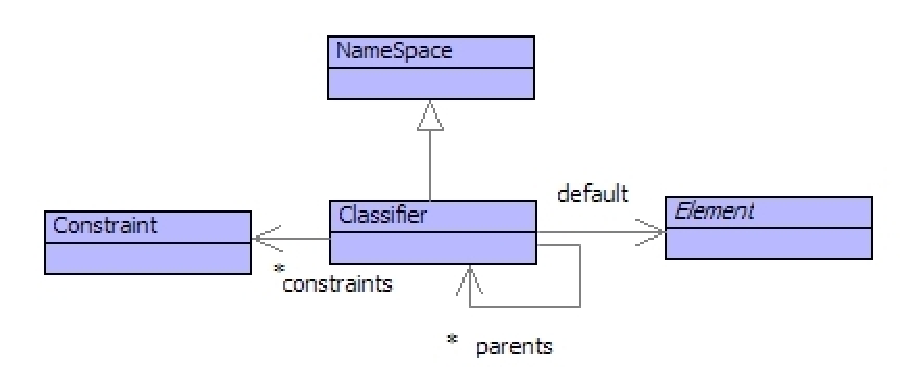
\includegraphics[width=12cm]{XMF/Languages/Images/Classifier.pdf}\hfill{}

\caption{Classifiers\label{fig:Classifiers}}

\end{center} \end{figure}


The values in a value domain fall into different groups: the integers,
the objects, the personnel records, the update events etc. Each of
these groups is a type and there is an element that represents the
type: a \emph{classifier}. A classifier is a single value that defines
characterising features of a group of values: its instances. Each
instance in the group refers to the classifier as its type. For example
the integer 3 has Integer as its type. Furthermore, sub-groups can
often be identified such that elements of a sub-group have more characterising
features - this is specialization.

Figure \ref{fig:Classifiers} shows the classes that define classification.
A classifier defines a collection of constraints: rules that govern
the characterising features of its instances. A classifier has parents,
the child parents are spcializations of the parent classifiers. All
the constraint rules of the parents are used to classify the instances
of the child classifier which may add rules of its own. Finally, a
classifier has a default element, for example the classifier Integer
has a default value of 0.

Classifier defines the following operations:

\begin{lstlisting}
Classifier::new()
  // Return a new instance of the receiver.
Classifier::new(args:Seq(Element))
  // Return a new instance of the receiver
  // after it is initialized using the args.
Classifier::invoke(target,args:Seq(Element))
  // Same as using new.
\end{lstlisting}
Each element in figure \ref{fig:Classifiers} is a classifier. For
example NameSpace classifies all name spaces in the value domain such
that a name space must have a collection of named elements and must
itself be a named element. It is always possible to ask an element
in the value domin what its classifier is. The operation Element::of()
returns a classifier; since this is provided by Element which classifies
everything, then all values in the domain support this operation.

%
\begin{figure} \begin{center}
\hfill{}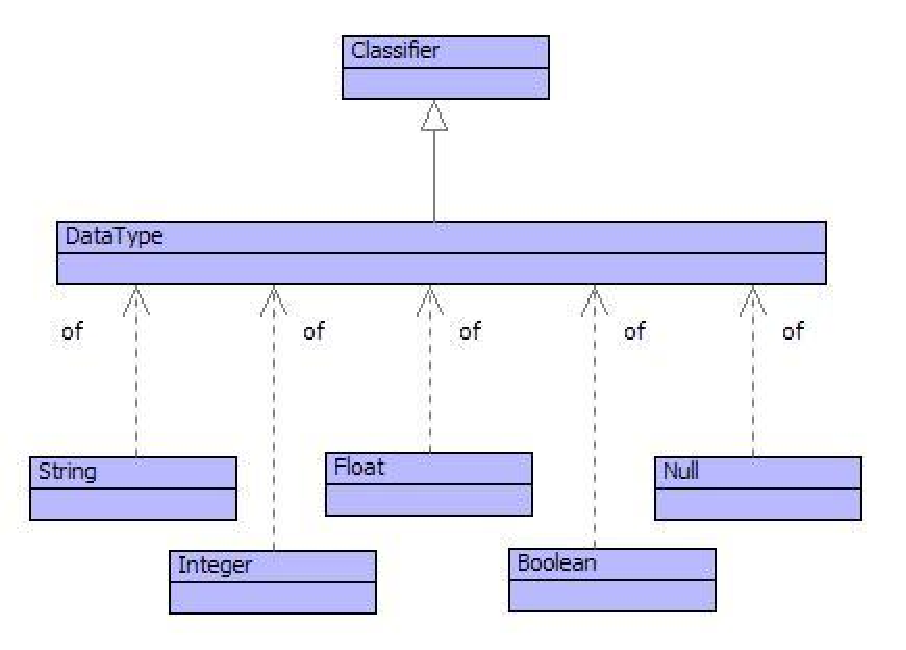
\includegraphics[width=12cm]{XMF/Languages/Images/DataType.pdf}\hfill{}

\caption{DataTypes\label{fig:DataTypes}}

\end{center} \end{figure}


The basic data values such as 10, true and {}``a string'' are all
classified by distinguished classifiers Integer, Boolean and string.
These classifiers, in turn are classified by the classifier DataType
as shown in figure \ref{fig:DataTypes}. The special value null is
classified by Null; it is used as the default value for all values
that have internal state.

The types String, Integer, Float, Boolean and Null each define their
own collection of operations that are listed in the appendix.


\section{Collections of Things}

%
\begin{figure} \begin{center}
\hfill{}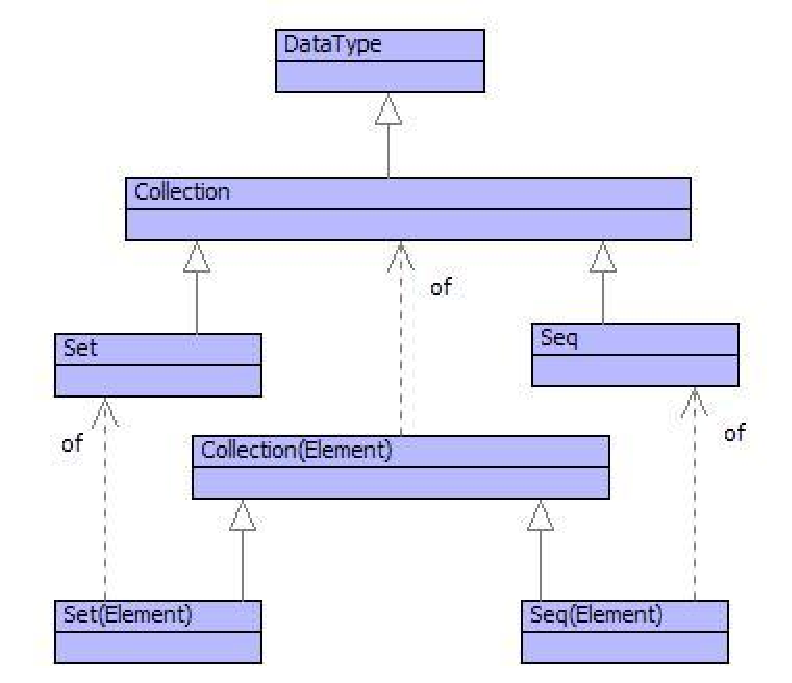
\includegraphics[width=12cm]{XMF/Languages/Images/Collections.pdf}\hfill{}

\caption{Collection Classifiers\label{fig:Collection-Classifiers}}

\end{center} \end{figure}


Two types of non-indexed collections are very useful: sets and sequences.
A set is an unordered collection, adding the same element to a set
has no effect and it is not possible to rely on the order of elements
in a set. The following is a set of integers: Set\{1,2,3,4\}, it is
the same set as Set\{4,3,2,1\} and the set Set\{1,1,3,2,3,4\}. Figure
\ref{fig:Collection-Classifiers} shows the classifiers that apply
to sets and sequences. In general the classifier of a set of elements
of type T is Set(T); since everything is classified by Element then
the most general set-based classifier is Set(Element).

%
\begin{figure} \begin{center}
\hfill{}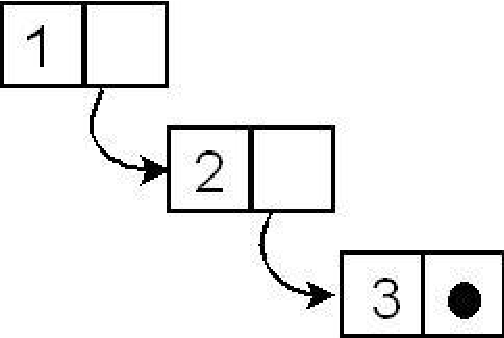
\includegraphics[width=5cm]{XMF/Languages/Images/Sequence.pdf}\hfill{}

\caption{A Sequence\label{fig:A-Sequence}}

\end{center} \end{figure}


A (non fixed size) sequence is either empty Seq\{\} or is a value
v followed by a sequence s: Seq\{v | s\}. A sequence has a head, v,
and a tail, s. Sequences lend themselves to recursive processing by
case analysis on the empty sequence and the non-empty sequence. Sequences
of elements of type T are classified by type Seq(T) and the most general
sequence classifier is Seq(Element).

Figure \ref{fig:A-Sequence} shows the sequence Seq\{1,2,3\} which
is equivalent to the sequence Seq\{1 | Seq\{2 | Seq\{3 | Seq\{\}\}\}\}.
The head of the sequence is the integer 1 and the tail of the sequence
is Seq\{2,3\}. The final dot in the figure represents the empty sequence
Seq\{\}.

Sequences of element are used heavily in this book to represent collections.
They are built-in to the implementation of the language and cannot
be extended. The appendix lists many of the operations that are provided
for manipulating sequences.


\section{Classifying Objects}

%
\begin{figure} \begin{center}
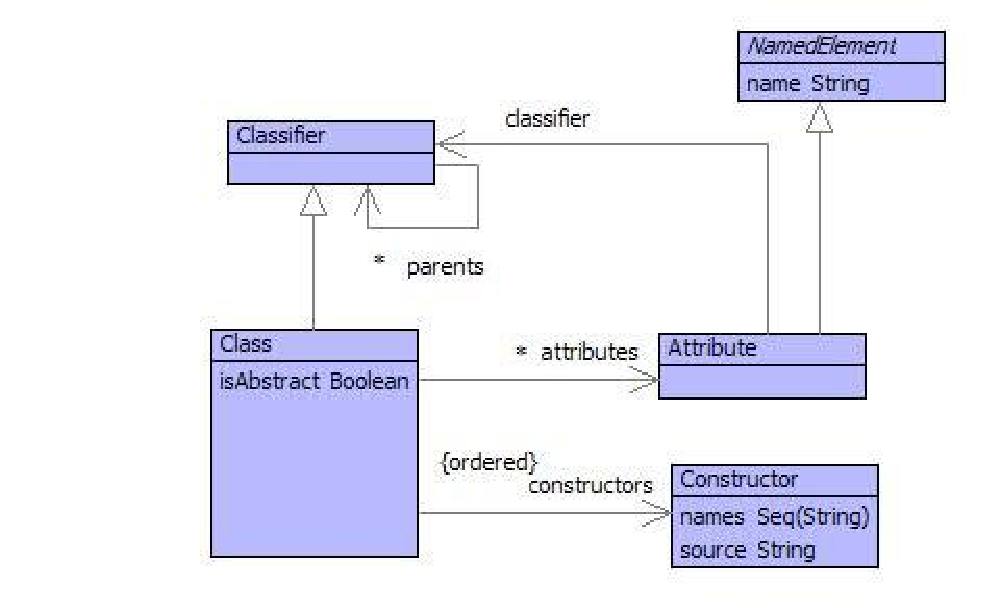
\includegraphics[width=12cm]{XMF/Languages/Images/Class.pdf}

\caption{Classifying Objects\label{fig:Classifying-Objects}}

\end{center} \end{figure}


Objects are values with identity and state. The identity is set when
the object is created and the state is represented as a collection
of slots. Each slot has a name and a value. Objects are used to represent
elements with properties, for example personnel records have personnel
properties including the name of the employee, salary and department.
Objects can be used to represent real-world things such as companies
or products and can be used to represent abstract things such as colours
(with red, green and blue properties) and system models.

Figure \ref{fig:Classifying-Objects} shows the classes that are used
to classify objects. The classifier of an object is a class with attributes
that classify the slots of the object. Each attribute has a name (defining
the name of the slot that the attribute classifies) and a type that
classifies the value of the slot. A class may be abstract in which
case it does not directly classify any objects, but may have sub-classes
(linked via the parents attribute from Classifier) whose direct instances
it classifies.

Each class has a number of constructors. Each constructor is a rule
that defines how a new instance of the class is created. A constructor
has a sequence of names that must correspond to the names of the attributes
defined (or inherited) by the class. When a constructor is used to
create an instance of a class it is supplied with values for each
of its names. A new instance of the class is created and the slots
with the corresponding names are initialized from the supplied values.
Each new instance will have a new identity. Constructors are inherited
from the parents of a class and there is always a constructor (inherited
from Object) that has no names.

For example, you can create a new object using a basic constructor
with no arguments as:

\begin{lstlisting}
Object()
\end{lstlisting}
The constructor for class (inherited from named element) allows a
new class to be constructed by supplying a name:

\begin{lstlisting}
Class("Animal")
\end{lstlisting}
The constructor for Table allows you to supply the approximate number
of elements to be stored in the table:

\begin{lstlisting}
Table(100)
\end{lstlisting}
\section{Performing Things}

The domain described so far contains elements that represent data,
but nothing that actually \emph{does} anything. It is possible to
inspect the value of an object's slot and update it, but there is
no domain element that represents what happens when an object receives
a message. the value domain contains operations that, upon being supplied
with argument values, perform actions. The actions that can be performed
are described in the next section; this section describes the basic
structure of an operation.

%
\begin{figure} \begin{center}
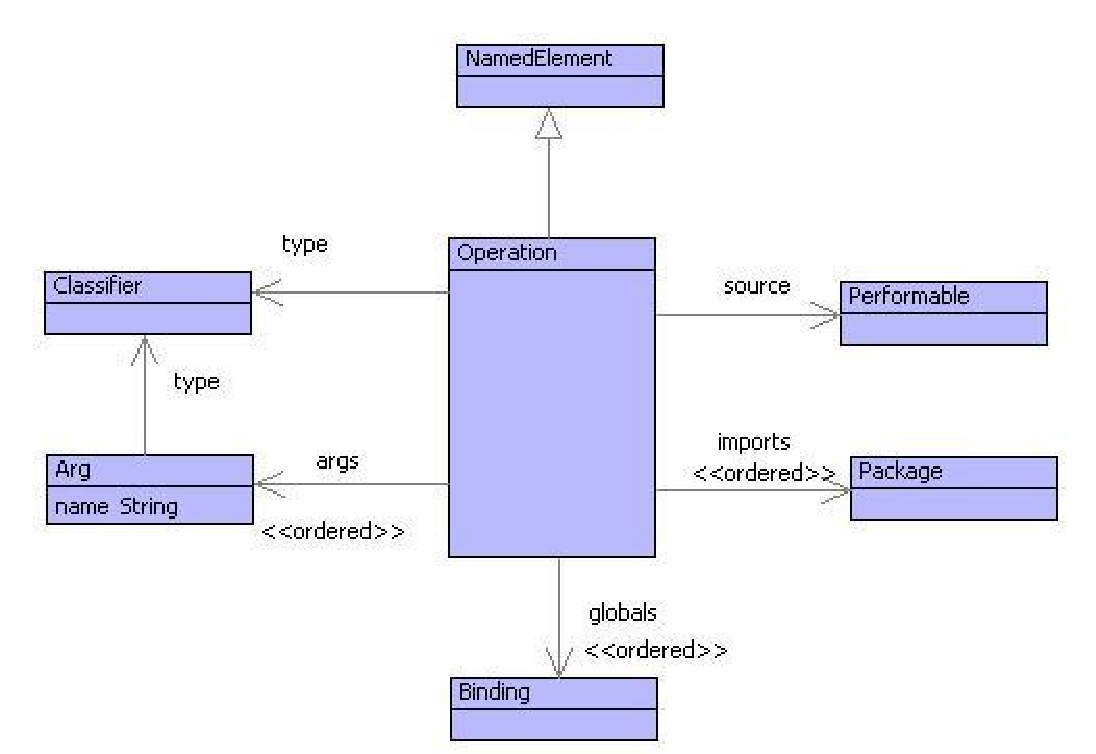
\includegraphics[width=12cm]{XMF/Languages/Images/Operation.pdf}

\caption{Operations \label{fig:Operations}}

\end{center} \end{figure}


Figure \ref{fig:Operations} shows the classes that define the tructure
of an operation. Each operation is a named element that can be placed
into a name space. An operation has a return type and a sequence of
typed arguments. The source of an operation is a performable element;
this is the source code of the operation that is performed then the
operation is invoked. 

Within the source there may be variable references. A variable reference
may correspond to an argument, a name from an imported name space
(called a dynamic variable), or a variable that was in scope when
the operation was created (called a global variable). Each of these
categories of variable are described with respect to examples in the
next section.

Operations give us the ability to run programs. Furthermore, there
is no restriction on where an operation can live in the value domain:
operations may be placed as the values of slots, may be added to collections
or may be placed in tables. All data values have to come into existence
somehow: they are produced by performing the actions in an operation.
Even operations come into existence this way.

Operation defines the following operations:

\begin{lstlisting}
Operation::arity():Integer
  // The number of arguments.
Operation::fork()
  // Start a new thread by calling the operations.
Operation::invoke(target,args:Seq(Element))
  // Call the operation with the target and args.
Operation::sig():Seq(Element)
  // Return the type signature of the operation.
Operation::source():String
  // Return the source code of the operation.
Operation::trace()
  // Trace calls of the operation.
Operation::untrace()
  // Opposite of trace.
\end{lstlisting}
